% Oliver Chi, draft for research project
% 1/9/2018
%
\documentclass[runningheads]{llncs}
%
\usepackage{graphicx}
\usepackage{amsfonts}
\usepackage[linesnumbered,lined,boxed,commentsnumbered]{algorithm2e}
\usepackage[utf8]{inputenc}
\usepackage{mathtools}
\makeatletter
\makeatother
%
%
%
%
\begin{document}
%
\title{Transfer Learning for Depression Detection on Social Networks\thanks{Supported by School of Information System, University of Southern Queensland, Australia}}
%
%
\author{Oliver Chi\inst{1}\and
Xiaohui Tao\inst{1} }
%
%
\institute{School of Information System, University of Southern Queensland, Australia\\
\email{\{ochi,xtao\}@usq.edu.au}}
%
\maketitle
%
\begin{abstract}
The abstract should briefly summarize the contents of the paper in
150--250 words.
%
\keywords{psychological knowledge base \and supervised learning \and depression.}
\end{abstract}
%
%
%
\pagebreak
\section{Introduction}
%
%
%
\pagebreak
\section{Related Work}
%
%
\subsection{Psychological Proposes}
%
%
\subsection{Psychological Proposes}
%
%
\pagebreak
\section{Definitions/Research Problem}
%
%
\paragraph{}
.... The research objective is defined:\\
\textbf{Definition 1} \textit{Let $\mathbb{S}$ be a set of user properties to present an effective user profile for depression, a user property s $\in$ $\mathbb{S}$ is a tuple s := $\langle$ p{\tiny{1}}, p{\tiny{2}}, p{\tiny{3}}, $\cdots$ p{\tiny{n}} $\rangle$, where
\begin{itemize}
  \item p is a visualisation or instance of an user property;
  \item p is not a mental or depression close-related symptom;
  \item n could be an infinite integer so the number of p elements could be unlimited;
  \item all p elements in the same user profile are generally independent.
\end{itemize}
}
%
%
\paragraph{}
With clear definition of research objective, the research target is defined:\\
\textbf{Definition 2} \textit{Let $\mathbb{V}$ be a set of labeled user depression, a label of user depression v $\in$ $\mathbb{V}$ is a screening result of personal depression, where
\begin{itemize}
  \item when v is binary, it presents depression (1) or healthy (0);
  \item when v is scale, it presents the severity of depression from healthy (0) to most severe depression(1).
\end{itemize}
}
%
%
\paragraph{}
From Definition 1, any given user property s $\in$ $\mathbb{S}$ is possibly overlapped with other user properties. The overlapped information in user profile apparently doesn't suit for classification. While learning from related psychological researches, a set of user personal functionings can present a perfect reflection of user mental profile. 
It innovates a creative method that detecting user depression by analysis of a set of user functionings. Therefore, the research problem is defined:\\
\textbf{Definition 3} \textit{Let $\mathbb{U}$ = $\langle$ u{\tiny{1}}, u{\tiny{2}}, u{\tiny{3}}, $\cdots$ u{\tiny{k}} $\rangle$ be a subset of $\mathbb{S}$, any element u $\in$ $\mathbb{U}$ is a tuple u := $\langle$ p'{\tiny{1}}, p'{\tiny{2}}, p'{\tiny{3}}, $\cdots$ p'{\tiny{n'}} $\rangle$,where
\begin{itemize}
  \item $\mathbb{U}$ is a machine-learning descriptive subset transferred from $\mathbb{S}$ in psychological domain descriptive;
  \item every p' $\in$ u is assigned from a instance p $\in$ s in Definition 1;
  \item $|\mathbb{D}^s|$ is limited due to the limited functionings defined in psychological domain.
\end{itemize}
This research aims to discover an effective classification model $\mathbb{M}$ which provides a reliable mapping of a well-defined $\mathbb{U}$ into $\mathbb{V}$: \\
\begin{center}
	$\mathbb{U}$ $\xRightarrow{\text{$\mathbb{M}$ } }$ $\mathbb{V}$  or  $\mathbb{M}$($\mathbb{U}$) = $\mathbb{V}$
\end{center}
}
%
%
\paragraph{}
%
%
%
\pagebreak
\section{Framework}
%
%
Therefore, the research problem is decomposed into two tasks: 
\begin{enumerate}
  \item data processing;
  \item modelling.
\end{enumerate}
%
\subsection{Conceptual Design}
%
%
whole framework
%
transfer knowledge:
data processing:
ensemble and modelling:
%
design standards, outcome
%
%
Driven by the processing of tasks, the conceptual framework of the proposed approach is designed consisting of three modules, as illustrated in Fig.~\ref{fig1}.
\begin{figure}[h]
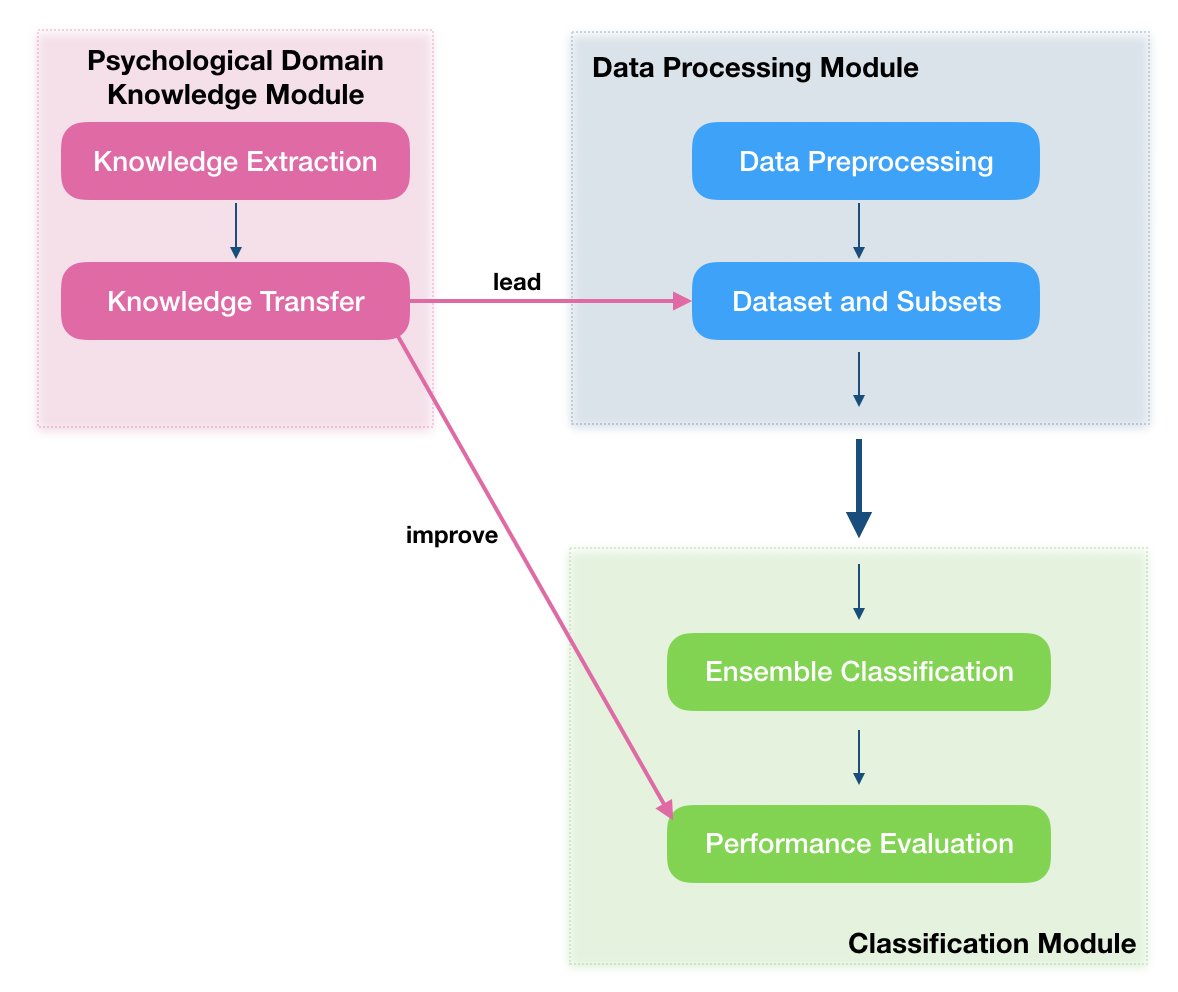
\includegraphics[width=1\textwidth]{concepts.png}
\caption{Conceptual Framework} \label{fig1}
\end{figure}
%
%
\subsection{Psychological Knowledge Base}
%
\paragraph{Psychological Domain Knowledge}
Kroenke et, al. [102] concluded that there was a strong association between increasing depression severity screen scores and worsening functionality on all 6 function: mental, social, role, pain, physical and overall functions. Other psychological researchers [103][104][105] also delivered similar opinion on the relation between depression and functions. 
%
\paragraph{Transfer Domain}
We hence can transfer psychological domain knowledge to information domain. \textit{$|\mathbb{D}^s|$} can be narrowed down to 6. The dataset of user mental profile is redefined:\\
\textbf{Definition 4} \textit{ Let new redesigned $\mathbb{U}$ = $\langle$ u{\tiny{mental}}, u{\tiny{social}}, u{\tiny{role}}, u{\tiny{pain}}, u{\tiny{physical}}, u{\tiny{overall}} $\rangle$, every u  $\in$ $\mathbb{U}$ is an independent function of user, where
\begin{itemize}
  \item u{\tiny{mental}} presents mental function;
  \item u{\tiny{social}} presents social function;
  \item u{\tiny{role}} presents role function;
  \item u{\tiny{pain}} presents pain function;
  \item u{\tiny{physical}} presents physical function;
  \item u{\tiny{overall}} presents the overall function.
\end{itemize}
}
%
%
\subsection{Data Processing}
%
%
(see Fig.~\ref{fig2}).
%
\begin{figure}[h]
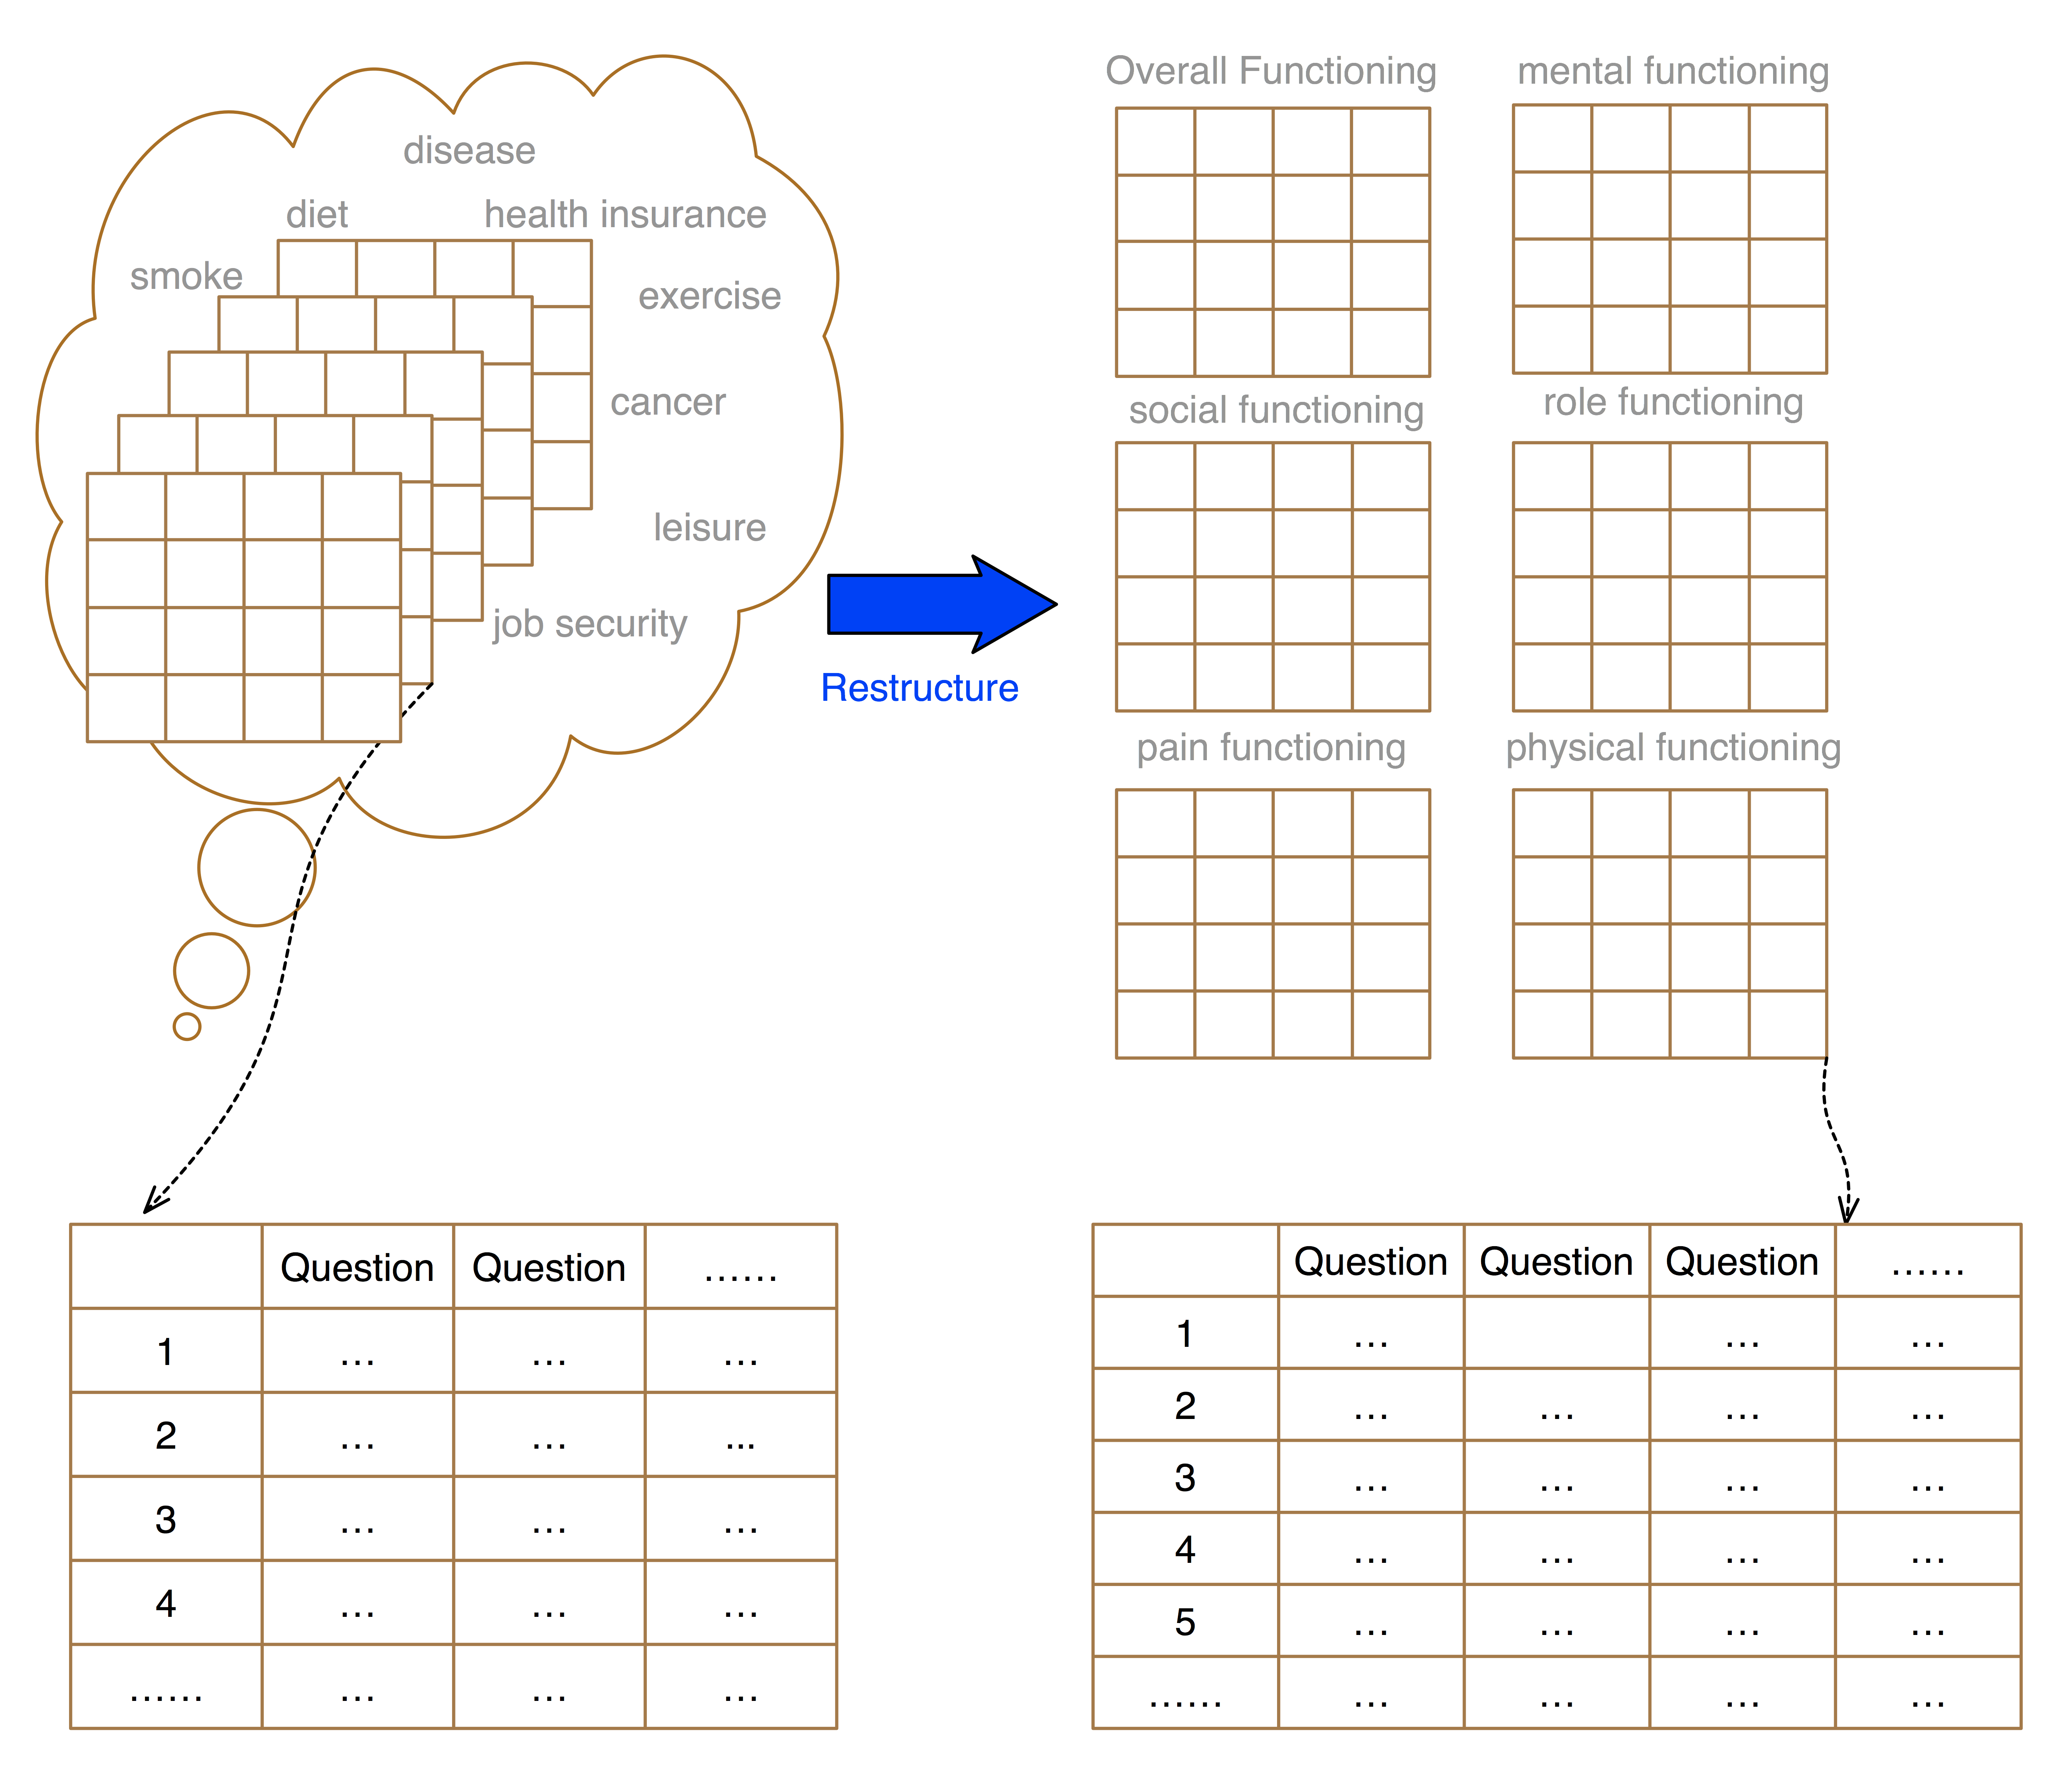
\includegraphics[width=0.8\textwidth]{restructure.png}
\caption{Data Restructure based on Psychological Knowledge Base} \label{fig2}
\end{figure}
%
\subsection{Modelling}
%
%
1. Design ensemble
2. Why ensemble
3. for each method, give technical purpose
4. model
5. Algorithm
%
Given a health dataset $i$ = $\langle$ u{\tiny{mental}}, u{\tiny{social}}, u{\tiny{role}}, u{\tiny{pain}}, u{\tiny{physical}}, u{\tiny{overall}} $\rangle$, \\
%
%
\IncMargin{1em}
\begin{algorithm}
	\SetKwData{Left}{left}\SetKwData{This}{this}\SetKwData{Up}{up}
	\SetKwFunction{Union}{Union}\SetKwFunction{FindCompress}{FindCompress}
	\SetKwInOut{Input}{input}\SetKwInOut{Output}{output}
		\Input{$i$ = $\langle$ u{\tiny{mental}}, u{\tiny{social}}, u{\tiny{role}}, u{\tiny{pain}}, u{\tiny{physical}}, u{\tiny{overall}} $\rangle$}
		\Output{ensemble modol}
		\BlankLine
		\emph{special treatment of the first line}\;
		\lForEach{element $e$ of the line $i$}{\FindCompress{p}}
	\caption{Ensemble}\label{algo_disjdecomp}
\end{algorithm}
\DecMargin{1em}
%
%
\pagebreak
\section{Experiment}
\subsection{Experiment Design}
\subsection{Dataset}
\subsection{Baseline Models}
\subsection{Performance Measure}
%
%
%
\pagebreak
\section{Results and Discussions}
\subsection{Experimental Results}
\subsection{Discussions}
%
%
\pagebreak
\section{Analysis}
\subsection{Sensitivity Study}
%
%
\pagebreak
\section{Conclusion and Future Work}
%
%
% ---- Bibliography ----
%
\begin{thebibliography}{8}
%\bibitem{ref_article1}		
%
\bibitem{ref_article101}	R. L. Spitzer, K. Kroenke, and J. B. Williams, "Validation and utility of a self-report version of PRIME-MD: the PHQ primary care study. Primary Care Evaluation of Mental Disorders. Patient Health Questionnaire," JAMA, vol. 282, no. 18, pp. 1737-44, Nov 10 1999.
%
\bibitem{ref_article102}	K. Kroenke, R. L. Spitzer, and J. B. Williams, "The PHQ-9: validity of a brief depression severity measure," J Gen Intern Med, vol. 16, no. 9, pp. 606-13, Sep 2001.
%
\bibitem{ref_article103}	M. Résibois, P. Kuppens, I. Van Mechelen, P. Fossati, and P. Verduyn, "Depression severity moderates the relation between self-distancing and features of emotion unfolding," Personality and Individual Differences, vol. 123, pp. 119-124, 2018.
%
\bibitem{ref_article104}	B. T. Stegenga et al., "Depression, anxiety and physical function: exploring the strength of causality," Journal of Epidemiology and Community Health, vol. 66, no. 7, pp. e25-e25, 2012.
%
\bibitem{ref_article105}	H. Xiao, J. Y. Yoon, and B. Bowers, "Living Arrangements and Quality of Life," Western Journal of Nursing Research, vol. 38, no. 6, pp. 738-752, 2015.
%
%
%
%
%
%
%
%
%
%
%
%
%
%
%
%
%
%
\end{thebibliography}
\end{document}
